Wir wollen unsere Werkzeuge zur Analyse von Signalen und Systemen nun um das wahrscheinlich wichtigste erweitern.
Hierbei zerlegen wir Signale, beziehungsweise Systemantworten/Impulsantworten, in ihre \q{harmonischen} Anteile -- wir transformieren in den \emph{Frequenzbereich}.
Man diese Art der \emph{Analyse} auch oft \emph{Fourier-Analyse}.
Da wir verschiedene Arten von Signalen bereits kennengelernt haben, muss diese Zerlegung auch auf verschiedene Weisen durchgef"uhrt werden.
F"ur diskrete Signale, ergibt es beispielsweise wenig Sinn, eine Integraltransformation zu definieren, Aperiodische Signale wiederum k"onnen nicht in einer Fourier-Reihe entwickelt werden, da die inh"arent der Periodizit"at widerspricht.
Das hei"st, dass f"ur jede \q{Art} von Signal und dessen Eigenschaften, die passende Transformation existiert.
Weiterhin "andert sich auch immer die \emph{Interpretation} dieser Zerlegung in harmonische Komponenten.

Dar"uber hinaus werden wir auch den umgekehrten Weg gehen.
Es ist auch m"oglich, Signale aus dem Frequenzbereich in den jeweils richtigen Definitionsbereicht zu transformieren. 
In diesem Fall spricht von von \emph{Fouriersynthese}, da wir ein Signal aus dessen Information "uber harmonische Anteile erzeugen/synthetisieren.
Wir liefern nun also die Definitionen und Zusammenh"ange der Fourier-Transformation, die wir in \Cref{sec:sampling} ohne Erl"auterungen ausgenutzt haben.

\subsection{Fourier-Transformation kontinuierlicher Signale}\label{sec:fourier:cont}

\subsubsection{Fourier-Transformation kontinuierlicher periodischer Signale}\label{sec:fourier:cont:period}

Wir haben bereits in \Cref{sec:cont_complex_harm} mit \eqref{eq:cont_fourier_series} gesehen, dass man durch Linearkombination der komplexen Sinus-Funktionen
\[
\{\exp(\jmath 2 \pi k F_0 t), \fuer k \in \Z\}
\]
eine $1/F_0=T_0$-periodische Funktion $x: \R \rightarrow \C$ durch
\[
x(t) = \Sum{k \in \Z}{}{c_k \exp(\jmath 2 \pi k F_0 t)}
\]
erh"alt.
Dies ist demnach ein Fall von \emph{Fourier-Synthese}, da wir aus den Gewichten $c_k$ in der Linearkombination eine Funktion $x$ erhalten.
Wir wollen nun den umgekehrten Weg gehen, auf welchem wir f"ur eine gegebene Funktion $x$ die Koeffizienten $c_k$ bestimmen k"onnen.
Wir starten dazu mit 
\begin{equation}\label{eq:fourier:fourier_series}
    x(t) = \Sum{k \in \Z}{}{
        c_k \exp(\jmath 2 \pi k F_0 t)
    }
\end{equation}
und multiplizieren beide Seiten mit $\exp(-\jmath 2 \pi \ell F_0 t)$ und integrieren "uber eine Periode $[0,T_0]$.
Dann erhalten wir
\[
\Int{0}{T_0}{
    x(t) \exp(-\jmath 2 \pi \ell F_0 t)
}{t} 
= \Int{0}{T_0}{
    \left(
        \Sum{k \in \Z}{}{
            c_k \exp(\jmath 2 \pi k F_0 t)
        }
    \right)
    \exp(-\jmath 2 \pi \ell F_0 t)
}{t} 
\]
und nach Vertauschung von Summation und Integration, dass
\[
\Sum{k \in \Z}{}{
    c_k 
    \Int{0}{T_0}{\exp(\jmath 2 \pi (k - \ell) F_0 t)}{t}
}
= \Sum{k \in \Z}{}{
    c_k \left[
        \frac{
            \exp(-\jmath 2 \pi (k - \ell) F_0 t)
        }{
            \jmath 2 \pi F_0(k - \ell)
        }
    \right]_{0}^{T_0}
}.
\]
Da die Funktion $\exp(-\jmath 2 \pi (k - \ell) F_0 t)$ im Fall $k \neq  \ell$ Periode $T_0$ besitzt, sind alle Summanden in der rechten Summation identisch $0$, au"ser wenn $k = \ell$.
Dann ergibt sich f"ur $\exp(\jmath 2 \pi (k - \ell) F_0 t) = 1$, also
\[
\Int{0}{T_0}{\exp(\jmath 2 \pi (k - \ell) F_0 t)}{t} 
    = \Int{0}{T_0}{1}{t} 
    = T_0.
\]
Final erhalten wir f"ur die Berechnung der Fourier-Koeffizienten $c : \N \rightarrow \C$ als Berechnungsvorschrift
\[
    c[\ell] = \frac{1}{T_0}\Int{0}{T_0}{
        x(t) \exp(-\jmath 2 \pi \ell F_0 t)
    }{t}.
\]
Wir haben in diesem Fall also \emph{Fourier-Analyse} betrieben.
Au"serdem haben wir absichtlich die Schreibweise von $c_\ell$ auf $c[\cdot]$ angepasst, um zu verdeutlichen, dass man nun die $c[\cdot]$ als \emph{komplexes diskretes Signal} auffassen k"onnen.
Dieses diskrete Signal k"onnen wir nun durch die Fourier-Reihe mit dem Signal $x : \R \rightarrow \C$ \emph{identifizieren}.
Sowohl $x$ als auch $c[\cdot]$ sind also Darstellungen desselben Sachverhaltes -- im \q{Zeitbereich} und im zugeh"origen \q{Frequenzbereich}.
Wir sehen auch, dass sich f"ur kontinuierliche und periodische Signale ein \emph{diskreter} Frequenzbereich ergibt.

Obige Herleitung verschleiert aber einen viel tiefer liegenden Zusammenhang.
Definieren wir wie in \Cref{sec:cont_complex_harm} die Funktionen $x_k : \R \rightarrow \C$ als
\[
x_k(t) = \exp(\jmath 2 \pi k F_0 t),
\]
dann k"onnen wir obige Rechnung auch so auffassen.
Wir betrachten Multiplikation von $x$ mit $x_\ell^\ast$ und anschlie"sende Integration als Skalarprodukt $\ScPr{x}{x_\ell}$. 
Au"serdem haben wir aus der Fourier-Reihe gegeben, dass
\[
x = \Sum{k \in \Z}{}{c_k x_k}
\]
Wir haben also in dieser Denkweise lediglich auf beiden Seiten der Fourierreihe in \eqref{eq:fourier:fourier_series} das Skalarprodukt mit $x_\ell$ gebildet.
Also
\[
\ScPr{x}{x_\ell} = \ScPr{\Sum{k \in \Z}{}{c_k x_k}}{x_\ell}.
\]
Das Skalarprodukt ist linear, also k"onnen wir auch
\[
\ScPr{x}{x_\ell} = \Sum{k \in \Z}{}{c_k \ScPr{x_k}{x_\ell}}
\]
schreiben.
Wir m"ussen also nur $\ScPr{x_k}{x_\ell}$ bestimmen. 
Dies haben wir aber oben schon berechnet, denn das waren die Ausdr"ucke
\[
\ScPr{x_k}{x_\ell}
    = \Int{0}{T_0}{x_k(t) x_\ell(t)^\ast}{t}
    = \Int{0}{T_0}{\exp(\jmath 2 \pi k F_0 t) \exp(-\jmath 2 \pi \ell F_0 t)}{t}
    = \Int{0}{T_0}{\exp(\jmath 2 \pi (k - \ell) F_0 t)}{t}
\]
Von oben wissen wir, dass
\[
\ScPr{x_k}{x_\ell} 
    = \left[
        \frac{
            \exp(-\jmath 2 \pi (k - \ell) F_0 t)
        }{
            \jmath 2 \pi F_0(k - \ell)
        }
    \right]_{0}^{T_0}
    = \begin{cases}
        T_0 \fuer k = \ell \\
        0, \Text{sonst.}
    \end{cases}
\]
Die $x_k$ stehen also paarweise \emph{senkrecht/orthogonal} zu einander und es gilt $\ScPr{x}{x_\ell} = T_0$.
Sie bilden ein sogenannten \emph{Orthogonalsystem}.
H"atten wir $\hat{x}_k = x_k / \sqrt{T_0}$ definiert, w"urde sogar gelten $\ScPr{\hat{x}_k}{\hat{x}_k} = 1$ und die $\hat{x}_k$ bilden eine \emph{Orthonormalsystem}.

Wenn wir nun noch einmal obige Gleichung f"ur $\ScPr{x}{x_\ell}$ betrachten, finden wir
\[
\ScPr{x}{x_\ell} 
    = \Sum{k \in \Z}{}{c_k \ScPr{x_k}{x_\ell}}
    = T_0 c_\ell,
\]
weil alle Summanden durch die Orthogonalit"at verschwinden und nur im Falle von $k = \ell$ eben $T_0$ "ubrig bleibt.
Der Fourier-Koeffzient $c_\ell$ ergibt sich also als Skalarprodukt von $x$ mit dem zugeh"origen $x_\ell$.
Es ist wichtig zu sehen, dass wir nur f"ur die Berechnung von $\ScPr{x_k}{x_\ell}$ die spezielle Form der $x_k$ eingesetzt haben und sonst nur allgemein mit den Eigenschaften von Skalarprodukten gearbeitet haben.
Das hei"st, dass man ganz allgemein Signale \q{transformieren} beziehungsweise \emph{analysieren} kann, indem man sie als Summe von paarweise orthogonalen Signalen ausdr"uckt.
Die Fourier-Reihe ist nur ein Spezialfall von diesem allgemeinen Konzept!

\begin{listing}[h]
    \noindent
    \begin{minipage}{0.51\textwidth}
        \strut\vspace*{-\baselineskip}\newline
        \inputminted[firstline=10, lastline=44]{python3}{code/fourier_series.py}
    \end{minipage}%
    \begin{minipage}{0.48\textwidth}
        \strut\vspace*{-\baselineskip}\newline
        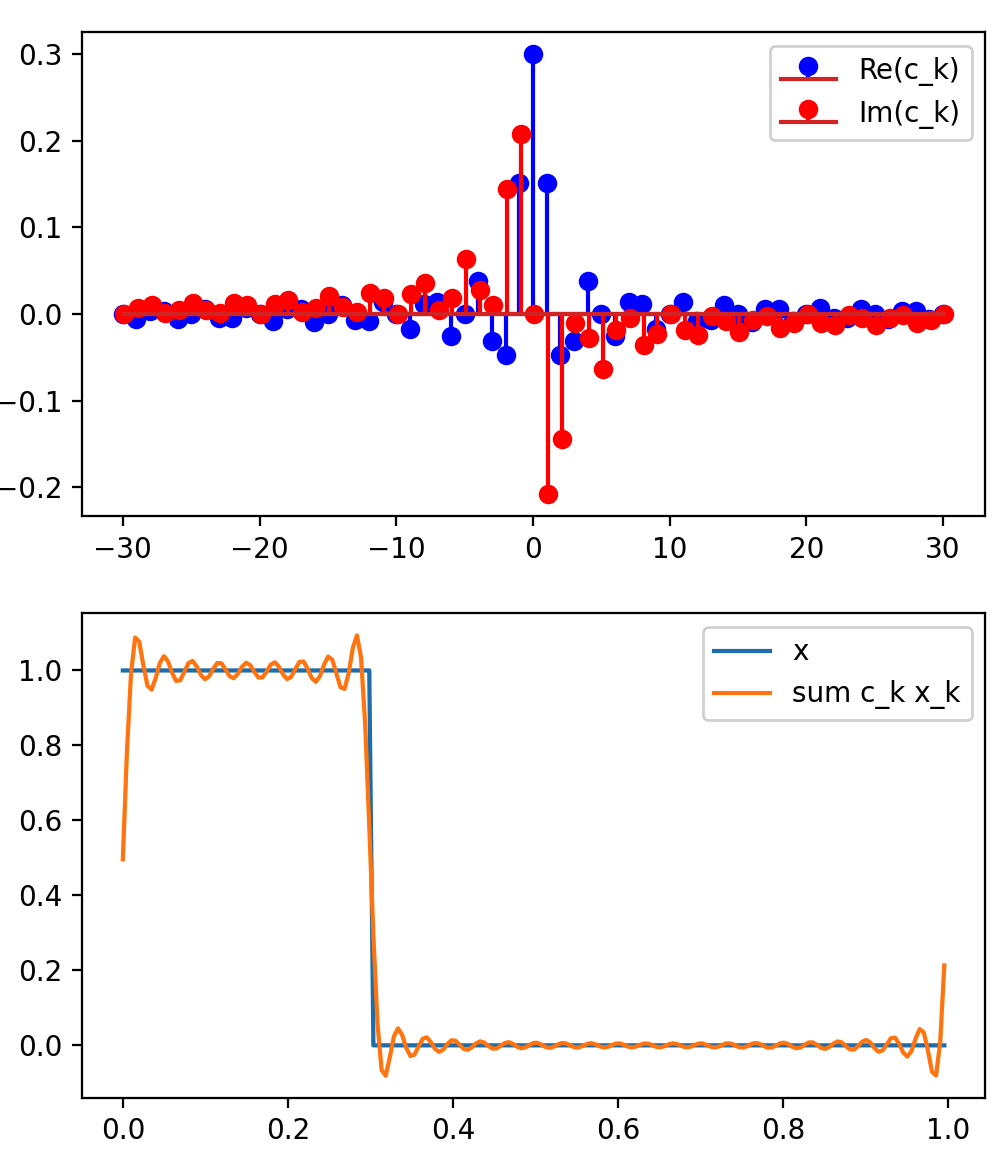
\includegraphics[width=\textwidth]{code/fourier_series.png}
    \end{minipage}
    \codecaption{dsv/code/fourier_series.py}{Berechnung und Darstellung von \eqref{eq:fourier:fourier_series}}\label{py:fourier_series}
\end{listing}

In \Cref{py:fourier_series} wird eine Rechteckfunktion $\Rect_{[0,T]}$ in ihre Fourier-Reihe entwickelt.
In diesem Fall m"ussen wir nat"urlich die Reihenentwicklung abbrechen, da kein $K_{\rm max}$ existiert, sodass $c[k] = 0$ f"ur $k > K_{\rm max}$.
Wir k"onnten die Reihe zwar analytisch ausrechnen, da wir jedes $x_k$ nur auf $[0,T]$ integrieren, also dem Bereich, auf dem die von uns definierte $\Rect_{[0,T]}$-Funktion Werte ungleich $0$ annimmt.
Der Einfachheit halber nutzen wir \texttt{scipy.integrate.quad}, was in der Lage ist numerische Integration relativ pr"azise durchzuf"uhren.

Es lohnt sich mit dem Wert von $K_{\rm max}$ zu experimentieren. 
Man sieht hierbei, dass gr"o"sere Werte von $K_{\rm max}$ an den Unstetigkeitsstellen $0$ und $T$ und in deren N"ahe nicht zu einer besseren "Ubereinstimmung der Fourierreiehe mit $x$ f"uhren.
Die Fourier-Reihe muss also nicht immer gegen $x$ konvergieren.
Im Falle von $\Rect_{[0,T]}$ ergibt sich das Problem genau aus dem Verhalten an $0$ und $T$ -- also Unstetigkeit, was ein generelles Problem bei der Entwicklung von Signalen in Fourier-Reihen darstellt.

Im oberen Plot von \Cref{py:fourier_series} sieht man auch, dass der Realteil der Koeffizienten $\Re{c[\cdot]}$ ein gerades diskretes Signal ist, also $c[k] = c[-k]$.
Der Imagin"arteil $\Im{c[\cdot]}$ hingegen ist ein ungerade Signal, also $c[k] = -c[-k]$\footnote{siehe \Cref{py:even_odd}}. 
Dies liegt daran, dass das Signal lediglich reelle Werte annimmt, weshalb die Symmetrie-Eigenschaften der $c[\cdot]$ allgemein f"ur reelle Signale gelten.

\begin{figure}
    \begin{center}
        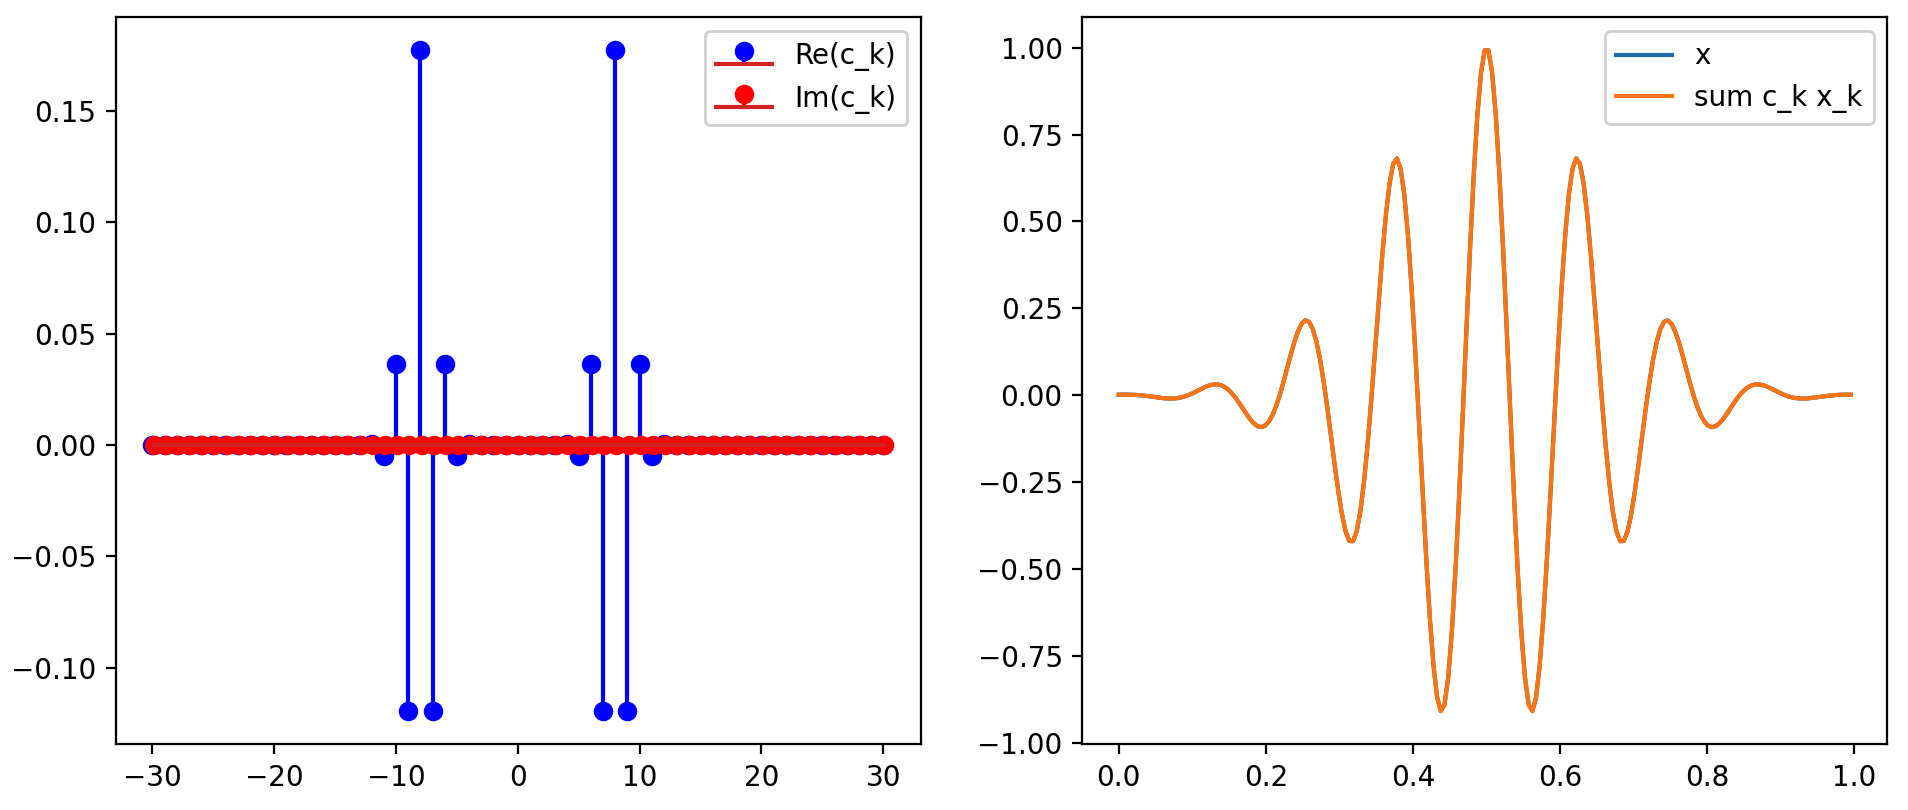
\includegraphics[width=0.8\textwidth]{code/fourier_series_1.png}

        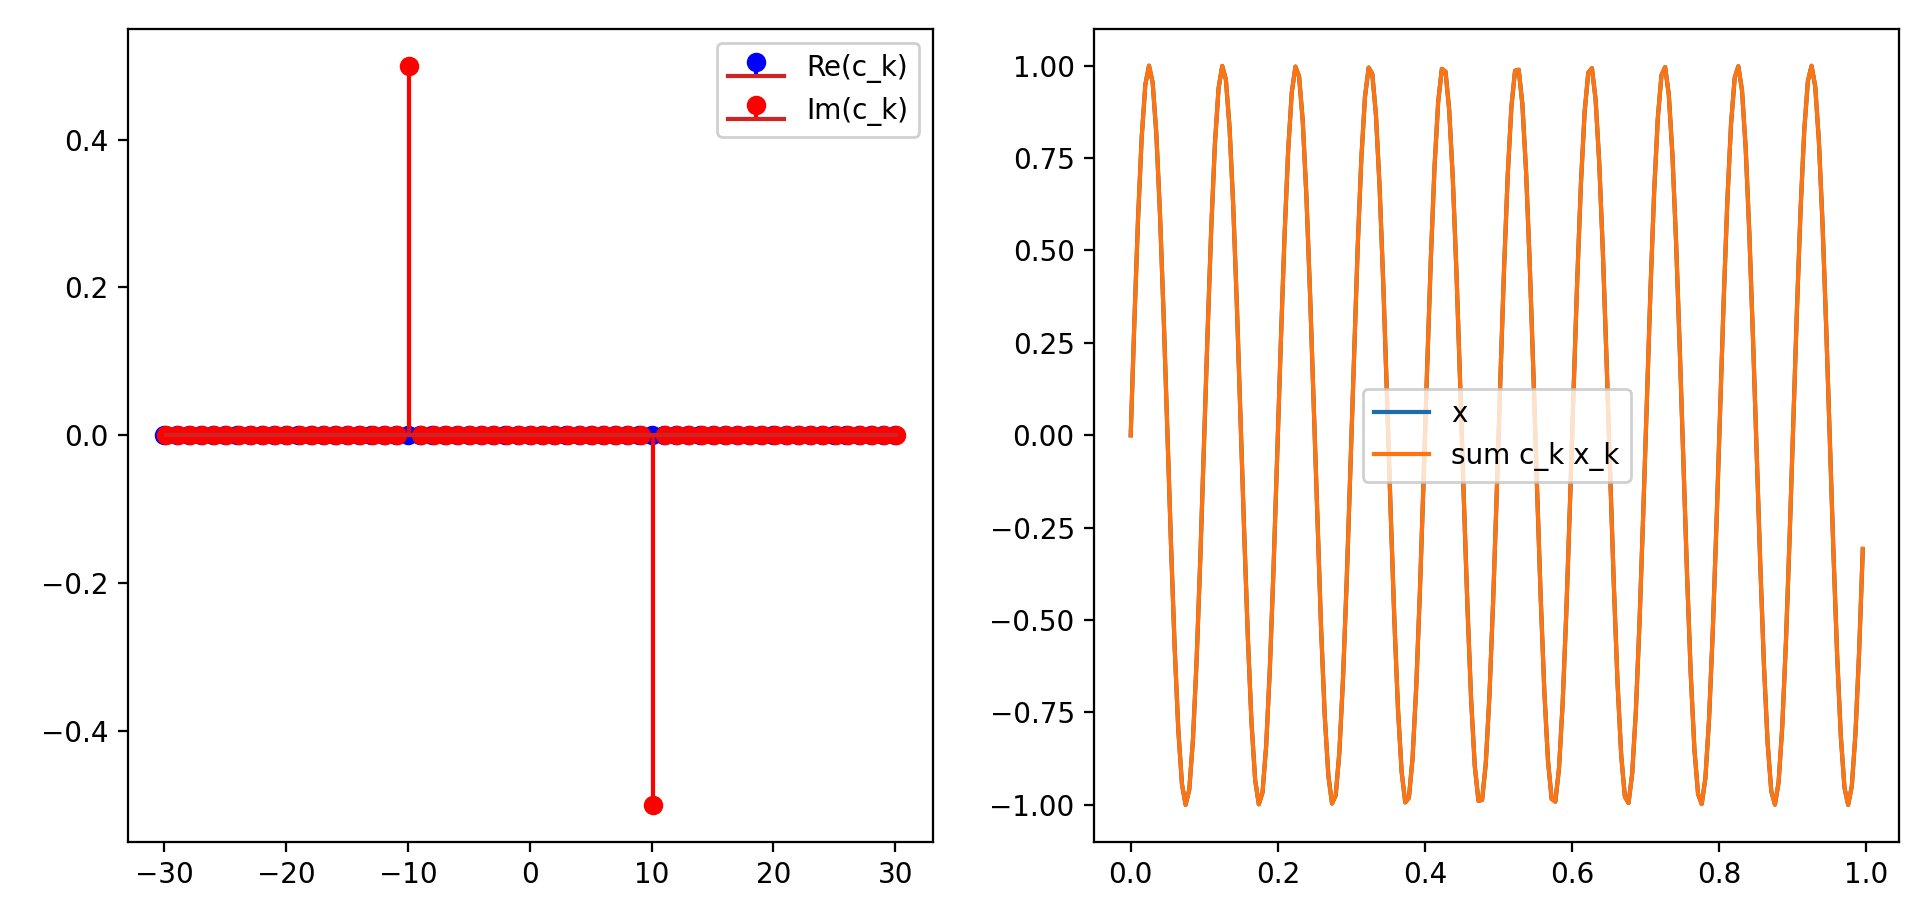
\includegraphics[width=0.8\textwidth]{code/fourier_series_2.png}
    \end{center}
    \caption{Mehr Versionen von \Cref{py:fourier_series}; Oben: $x(t) = \exp(-25(t-0.5)^2) \cos(16 \pi t)$; Unten: $x(t) = \sin(20 \pi t)$;}\label{fig:fourier:fourier_series}
\end{figure}

In \Cref{fig:fourier:fourier_series} sind noch mehr Eigenschaften der Fourier-Reihe deutlich gemacht.
Generell stellen wir fest, dass die beiden Signale jeweils gut durch eine endliche Fourier-Reihe approximiert werden k"onnen, da sie keine Unsteigkeiten aufweisen.
Im oberen Plot sieht man au"serdem, dass Achsen-Symmetrie des Signals $x$ dazu f"uhrt, dass die Imagin"arteile von $c[\cdot]$ verschwinden.
Wie man in \Cref{fig:fourier:fourier_series} unten sieht, ist es bei Anti-Symmetrie des Signals $x$ der Realteil von $c[\cdot]$, der verschwindet.
Dies liegt daran, dass der Realteil der $x_k$ eine gerade Funktion ist und der Imagin"arteil respektive eine ungerade Funktion.
Da wir in \Cref{py:even_odd} schon gesehen haben, dass ungerade und gerade Anteile eines Signals im Sinne von Skalarprodukten orthogonal sind, gilt dies auch f"ur die resultierenden Fourier-Koeffizienten.
In \Cref{fig:fourier:fourier_series} unten sieht man auch, dass man f"ur gewisse Signale die Fourier-Reihe direkt angeben kann.
Im Falle des Beispiels gilt n"amlich
\[
x(t) 
    = \sin(10 \cdot 2 \pi t) 
    = \frac{1}{2 \jmath} \left(
        \exp(10 \cdot 2 \pi t) + \exp(-10 \cdot 2 \pi t)
    \right) 
    = \frac{1}{2 \jmath} x_{10} + \frac{1}{2 \jmath} x_{-10}.
\]
Das hei"st, dass wir $x$ \emph{direkt} in seine Fourier-Reihe entwickelt haben, da wir es als Linearkombination der $x_k$ dargestellt haben.
Das hei"st es sind nur $x_{10}$ und $x_{-10}$ notwendig, um $x$ darzustellen und beide Koeffizienten haben ausschlie"slich imagin"are Anteile.

"Ahnlich wie bei der $z$-Transformation kann man also an der Fourier-Reihe Eigenschaften des Signals $x$ direkt ablesen, oder umgekehrt von Eigenschaften des Signals $x$ auf Eigenschaften der Fourier-Koeffizienten $c[\cdot]$ schlie"sen.
Au"serdem werden wir f"ur die noch folgenden Versionen der \gls{ft} sehr analoge Zusammenh"ange finden.

\subsubsection{Leichtungsdichte-Spektrum periodischer Signale}

Das Leichtungsdichtespektrum eines $T_0$-periodischen Signals $x: \R \rightarrow \C$ is gegeben durch
\begin{equation}\label{eq:fourier:period_psd}
P(x) = \frac{1}{T_0}\Int{0}{T_0}{\Abs{x(t)}^2}{t}
     = \frac{1}{T_0}\Int{0}{T_0}{x(t) x(t)^\ast}{t}
     = \frac{1}{T_0} \ScPr{x}{x}.
\end{equation}
Wir wollen nun $P(x)$ in Abh"angigkeit der Fourier-Koeffizienten $c[\cdot]$ berechnen.
Wir entwickeln also
\[
x(t) = \Sum{k \in \Z}{}{
    c_k \exp(\jmath 2 \pi k F_0 t)
}
\]
und setzen dies in $P$ ein, um
%
\begin{equation}\label{eq:fourier:series_parseval}
    \frac{1}{T_0}\Int{0}{T_0}{x(t) x(t)^\ast}{t}
        = \frac{1}{T_0}\Int{0}{T_0}{
            x(t) 
            \Sum{k \in \Z}{}{
                c_k^\ast \exp(-\jmath 2 \pi k F_0 t)
            }
        }{t}
        = \Sum{k \in \Z}{}{
            c_k^\ast 
            \frac{1}{T_0}\Int{0}{T_0}{
                x(t)
                \exp(-\jmath 2 \pi k F_0 t)
            }{t}
        }
        = \Sum{k \in \Z}{}{
            c_k^\ast c_k
        }
\end{equation}
%
als den \emph{Satz von Parseval}\footnote{\url{https://de.wikipedia.org/wiki/Satz\_von\_Parseval}} zu erhalten.
Die physikalische Interpretation ist, dass $\Abs{c[k]}$ der Leistung des Signals bei der Frequenz $k F_0$ entspricht.
Jeder Index $k$ hat also eine physikalische Gr"o"se, die mit ihm assoziiert ist.

Da nur die Frequenzen $k F_0$ f"ur $k \in \Z$ auftreten, also Frequenzen wie $0.1 F_0$ nicht vorhanden sind, sprechen wir von einem \emph{diskreten Spektrum}.
Es ergibt sich also direkt folgender wichtiger Zusammenhang: Periodische Signale im Zeitbereich besitzen ein \emph{diskretes} Spektrum.
Andersherum ergibt sich auch: Signale mit diskretem Spektrum sind periodisch.
Beide Argument ergeben sich aus der Fourier-Reihe.
Damit haben wir das duale Ergebnis zu \eqref{eq:spectrum_sampled} gefunden.
Dort f"uhrte Diskretisierung im Zeitbereich, also Sampling/Abtastung, zu einer Periodifizierung im Frequenzbereich.

\begin{listing}[h]
    \noindent
    \begin{minipage}{0.51\textwidth}
        \strut\vspace*{-\baselineskip}\newline
        \inputminted[firstline=5, lastline=14]{python3}{code/period_psd.py}
    \end{minipage}%
    \begin{minipage}{0.48\textwidth}
        \strut\vspace*{-\baselineskip}\newline
        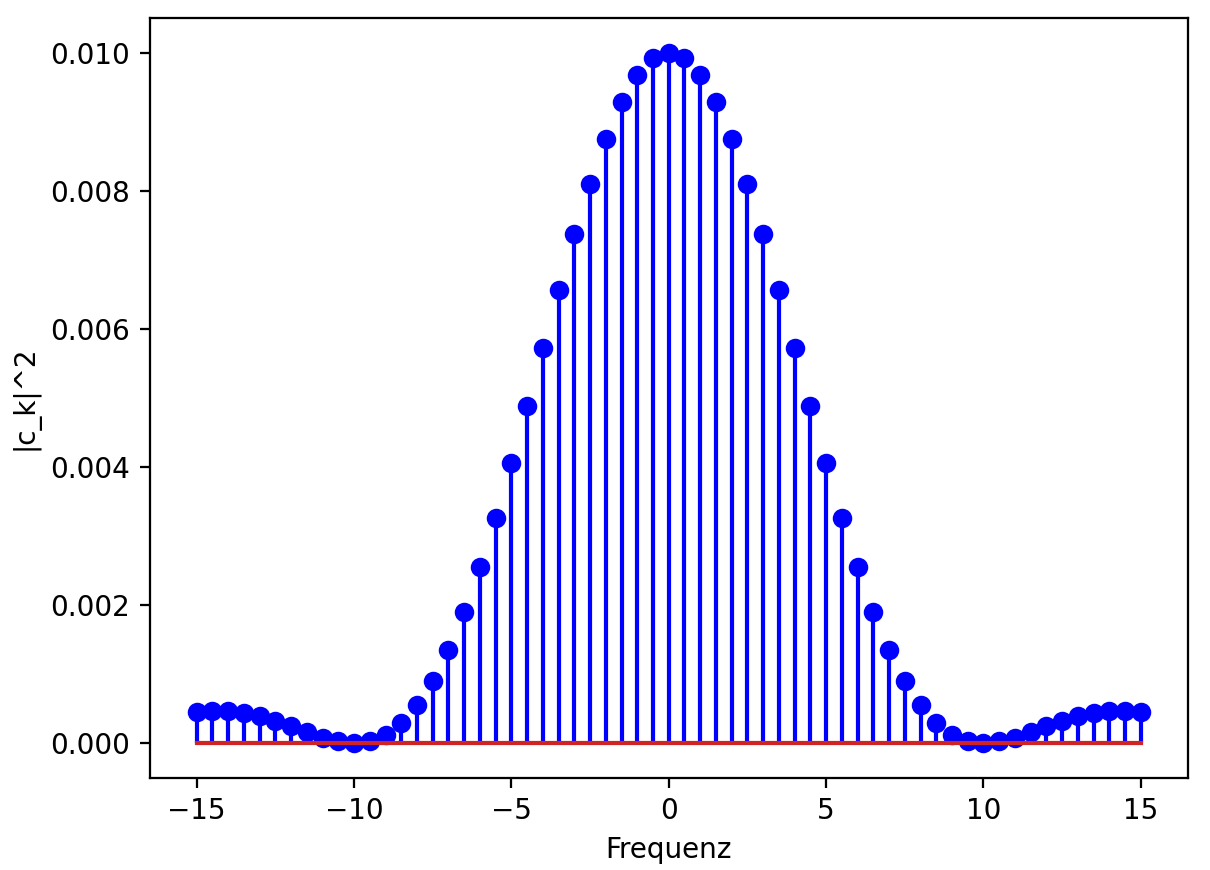
\includegraphics[width=\textwidth]{code/period_psd.png}
    \end{minipage}
    \codecaption{dsv/code/period_psd.py}{Modizifiertes \Cref{py:fourier_series} und Plot von $P$ im Frequenzbereich.}\label{py:period_psd}
\end{listing}

In \Cref{py:period_psd} zeigen wir eine Modifikation von \Cref{py:fourier_series}, in welcher wir $T_0 = 2$ setzen, also $F_0=1/2$ erhalten. 
Auf der Frequenzachse sehen wir, dass demnach diese f"ur $K_{\rm max} = 30$ also von $-15$ bis $+15$ reicht.
%
%
\FloatBarrier
\subsubsection{Fourier-Transformation von kontinuierlichen aperiodischen Signalen}
%
Um die Einschr"ankung auf periodische Signale zu vermeiden, nutzen wir die \acrlong{ft}, wie wir sie bereits in \eqref{eq:sampling:fourier_trafo} f"ur ein Signal $x : \R \rightarrow \C$ durch
\begin{equation}\label{eq:fourier:fourier_trafo}
    X(F) = \Int{-\infty}{+\infty}{x(t) \exp(-\jmath 2 \pi F t)}{t}
\end{equation}
definiert haben.
Im Unterschied zu \eqref{eq:fourier:fourier_series} integrieren wir nun "uber ganz $\R$, da sich das Signal nicht mehr periodisch wiederholt.
Aus diesem Grund ergibt sich auch ein \emph{kontinuierliches} Spektrum, da wir uns nicht mehr auf eine abz"ahlbare Menge von diskreten Frequenzen zur"uckziehen k"onnen.
Deshalb ergibt sich auch f"ur die Synthese des Signals, dass wir auch in diesem Fall integrieren anstatt summieren m"ussen, es gilt also
\begin{equation}\label{eq:fourier:inv_fourier_trafo}
    x(t) = \Int{-\infty}{+\infty}{X(F) \exp(\jmath 2 \pi F t)}{F}.
\end{equation}
Da sich f"ur die meisten Signale, die wir betrachten werden, Integration und Summation \q{"ahnlich} verhalten, finden wir auch die obigen Eigenschaften bez"uglich Symmetrien, etc., von \eqref{eq:fourier:fourier_series} wieder.

Es gibt aber eine Verbindung zur Fourier-Reihe, die wir im Folgenden kurz erl"autern wollen.
Nehmen wir an, es existiert ein $T > 0$, sodass $\Abs{x(t)} = 0$ f"ur alle $t$ mit $\Abs{t} > T$.
Dann k"onnen wir das Signal $x$ periodifizieren mit Periode $T$, indem wir
\[
x_p(t) = \Sum{k \in Z}{}{x(t - kT)}
\]
setzen.
Dies haben wir bereits in "ahnlicher Form in \eqref{eq:spectrum_sampled} gesehen. 
Dort hat es sich aber aus Berechnungen ergeben und hier \emph{setzen} wir diesen Zusammenhang explizit.
Dann k"onnen wir $x_p$ in seine Fourier-Reihe 
\[
x_p(t) = \Sum{k \in \Z}{}{c_k \exp(\jmath 2 \pi k t/T)}
\Text{mit}
T\,c_k = \Int{-T/2}{+T/2}{x_p(t) \exp(- \jmath 2 \pi k t/T)}{t}
    = \Int{-\infty}{+\infty}{x(t) \exp(- \jmath 2 \pi k t/T)}{t}
\]
entwickeln.
Aus der Definition in \eqref{eq:fourier:fourier_trafo} und der letzten Gleichung sehen wir, dass sich die Koeffizienten der Fourier-Reihe finden lassen durch
\begin{equation}\label{eq:fourier:c_k_fourier}
    c_k = \frac 1T X\left(\frac kT\right),
\end{equation}
diese sich also auch aus der Fourier-Transformation ablesen lassen.
Das hei"st, dass wir auch
\[
x_p(t) = \Sum{k \in \Z}{}{\frac 1T X\left(\frac kT\right) \exp(\jmath 2 \pi k t/T)}
       = \Sum{k \in \Z}{}{X\left(k \Delta F\right) \exp(\jmath 2 \pi k t \Delta F) \Delta F}
\]
schreiben k"onnen.
Dabei haben wir im letzten Schritt $1/T = \Delta F$ gesetzt.
Dies k"onnen wir intuitiv (aber nicht rigoros!) so interpretieren, dass im Falle von $T \rightarrow \infty$ gilt, dass $\Delta F \rightarrow 0$.
Je l"anger der Bereich der Funktion $x$, auf welchem gilt $x \neq 0$, desto kleiner $\Delta F$.
Der nicht-periodische Fall $T = \infty$ ergibt sich also als Grenzfall, bei welchem obige Summation zu einer Integration wird und $\Delta F$ zu einem $\mathrm{d}F$.
Man kann die \acrlong{ft} also als Grenzfall der Fourier-Reihe f"ur $T \rightarrow \infty$ betrachten.
%
%
\subsubsection{Leistungsdichte-Spektrum aperiodischer Signale}
%
Analog zum Satz von Parseval f"ur periodische Signale in \eqref{eq:fourier:series_parseval} k"onnen wir auch hier wieder definieren und folgern, dass
\begin{equation}
E(x) = \Int{-\infty}{+\infty}{\Abs{x(t)}^2}{t}
     = \Int{-\infty}{+\infty}{\Abs{X(F)}^2}{F}
\end{equation}
auch wieder ein Parseval Theorem f"ur die \acrlong{ft} ergibt.

Andererseits kann man $X$ auch in Betrag und Phase zerlegen, da es im Allgemeinen eine komplexe Gr"o"se ist, also
\[
X(F) = \Abs{X(F)} \exp(\jmath \angle(X(F))).
\]
Man nennt dann $\Abs{X(F)}^2$ das \emph{Leistungsdichte-Spektrum} von $x$.

\begin{listing}[h]
    \noindent
    \begin{minipage}{0.51\textwidth}
        \strut\vspace*{-\baselineskip}\newline
        \inputminted[firstline=6, lastline=45]{python3}{code/fourier_trafo.py}
    \end{minipage}%
    \begin{minipage}{0.48\textwidth}
        \strut\vspace*{-\baselineskip}\newline
        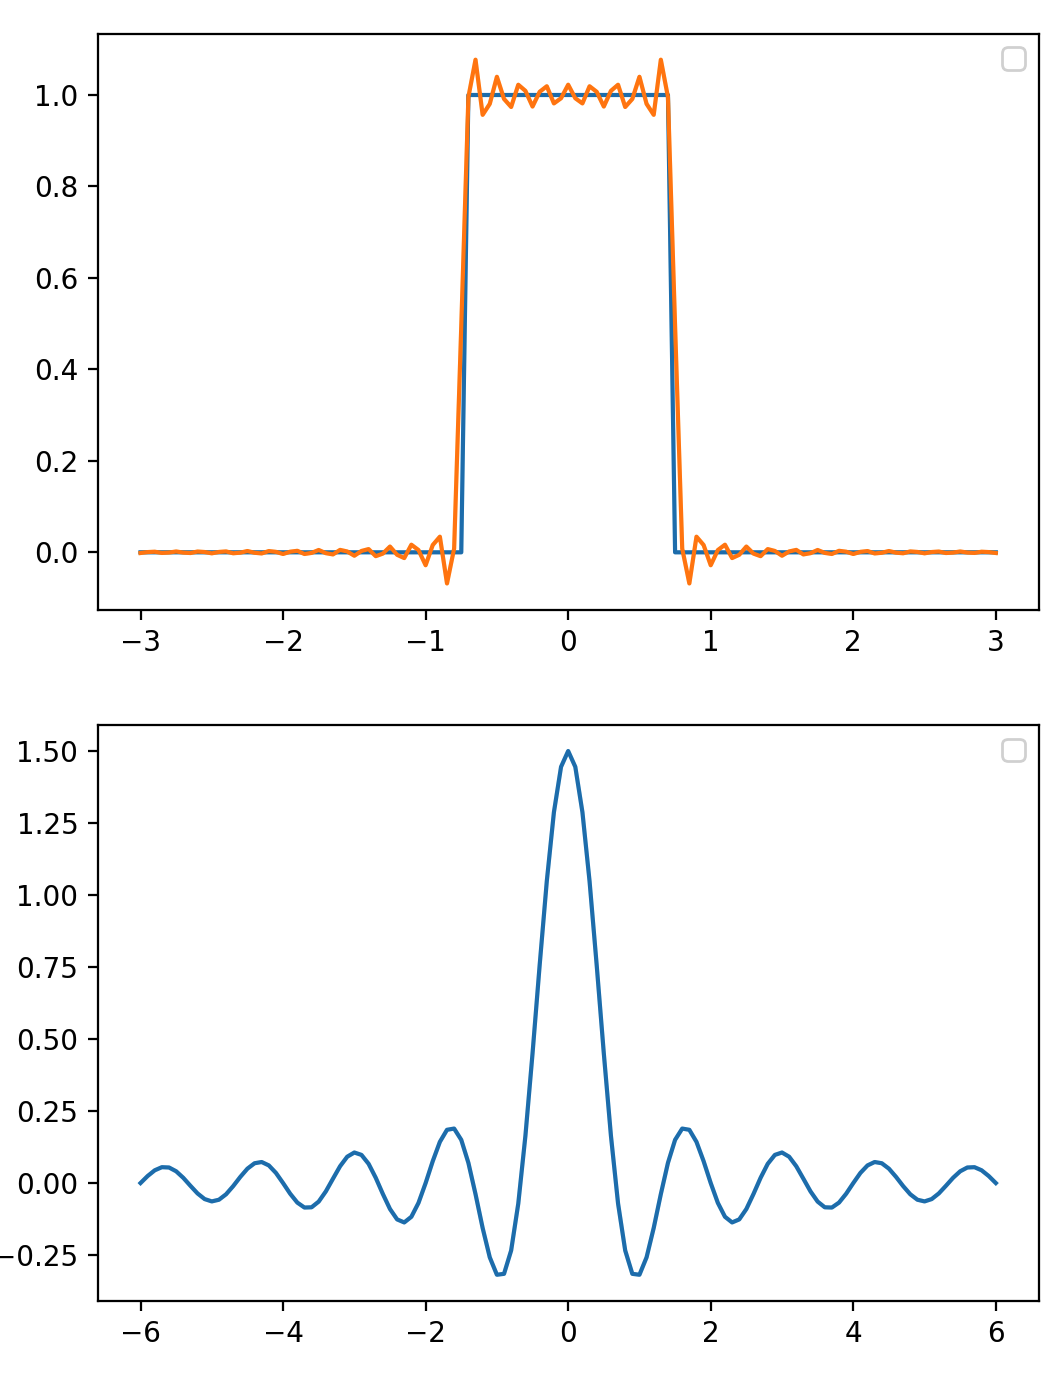
\includegraphics[width=\textwidth]{code/fourier_trafo.png}
    \end{minipage}
    \codecaption{dsv/code/fourier_trafo.py}{Berechnung und Darstellung von \eqref{eq:fourier:fourier_trafo}}\label{py:fourier_trafo}
\end{listing}

In \Cref{py:fourier_trafo} zeigen wir das Vorgehen zur Fourier-Analyse mittels numerischer Integration.
Es ist hier anzumerken, dass wir \q{nur} die Funktion \texttt{rect} definieren m"ussen und der Rest, also die Funktionen \texttt{kernel}, \texttt{analyse} und \texttt{synthese} unabh"angig hiervon sind.
Wir haben hier ein \namecref{py:fourier_trafo}, welches sich Methoden der Funktionalen Programmierung bedient.
Die Funktionen texttt{analyse} und \texttt{synthese} haben als Eingabewert die entweder die Funktion, oder die \acrlong{ft} einer Funktion.
Au"serdem liefern sie als Ausgabewert wieder \emph{Funktionen}, die wir einfach \q{aufrufen} k"onnen.
%
\subsection{Fourier-Transformation diskreter Signale}\label{sec:fourier:disc}
%
Wir n"ahern uns langsam der Fourier-Analyse von diskreten Signalen.
Schlie"slich wollen wir etwaige spektrale Analysen und dergleichen im Digitalen durchf"uhren, um die Vorz"uge von digitalen Rechenwerken dabei nutzen zu k"onnen.
Die vorher eingef"uhrten Transformationen sind zwar hilfreich f"ur theoretische Argumentation, wie beispielsweise beim Sampling-\Cref{stm:sampling_theorem}. 
Deshalb wenden wir uns nun der spektralen Analyse von diskreten Signalen zu.
Wir werden aber im Verlauf auch wieder "ahnliche Zusammenh"ange wie in \eqref{eq:fourier:c_k_fourier} finden.
%
\subsubsection{Fourier-Transformation diskreter periodischer Signale}\label{sec:fourier:dft}
%
Wir beginnen mit diskreten Signalen, die gleichzeitig periodisch sind, also ein $N$ existiert, sodass
\[
x[n] = x[n+N] \Text{f"ur alle} n \in \Z 
\]
gilt.
Aus vorherigen Diskussionen in \Cref{sec:sampling} wissen wir einerseits, dass diskrete Signale ein periodisches Spektrum auf $(0,1)$ besitzen.
Andererseits wissen wir aus \Cref{sec:fourier:cont:period}, dass periodische Signale ein \emph{diskretes} Spektrum besitzen.
Wir finden also nun intuitiv, dass das Spektrum von diskreten periodischen Signalen \emph{ebenfalls} diskret und periodisch ist.
Denken wir zur"uck an \Cref{sec:sampling:disc_sin} so haben wir bereits alles Notwendige betrachtet.
Ein $N$-periodisches diskretes Signal ergibt sich aus der Linearkombination der diskreten Signale $x_k[\cdot] : \Z \rightarrow \C$ definiert durch
\[
x_k[n] = \exp\left(\jmath 2 \pi \frac k N n \right) \Text{mit} k = 0, \ldots, N-1.
\]
Das hei"st, f"ur $x[\cdot]$ setzen wir mit
\[
x[\cdot] = \Sum{k = 0}{N-1}{c[k] x_k[\cdot]}
\]
an.
Damit sind bereits beide Eigenschaften des Spektrums \q{eingepreist}.
Denn man erkennt in den $x_{k}[\cdot]$ die vorher erw"ahnte \emph{zweifache} Periodizit"at wieder, weil sowohl $x_{k+N}[\cdot] = x_{k}[\cdot]$ f"ur alle $k$ als auch $x_k[n+N] = x_k[n]$ f"ur alle $n$ gilt.

Es ist nun unser Ziel f"ur gegebene Werte $x[n]$ von $x[\cdot]$ die Werte des \emph{ebenfalls periodischen und diskreten} Signals $c[\cdot]$ zu bestimmen.
Dies verl"auft ganz analog zu \Cref{sec:fourier:cont:period}.
Wir definieren das Skalarprodukt $\ScPr{\cdot}{\cdot}$ f"ur $N$-periodische und diskrete Signale via
\[
\ScPr{x_1[\cdot]}{x_2[\cdot]} 
    = \Sum{n = 0}{N-1}{x_1[n] x_2[n]^\ast}.
\]
Das hei"st, dass wir periodisches Signal $x[\cdot]$ mit dem \emph{endlich-dimensionalen} Vektor $\bm x \in \C^{N}$ identifizieren, wir setzen also die EIntr"age des Vektors als $\bm x_i = x[i-1]$.
Dann k"onnen wir auch f"ur das entsprechende Skalarprodukt der Vektoren $\bm x_{1,2} \in \C^N$
\[
\ScPr{\bm x_1}{\bm x_2} 
    = \left(\bm x_2^\ast\right)^\trans \cdot \bm x_1 
    = \bm x_2^\herm \cdot \bm x_1
\]
schreiben.
Analog identifizieren wir die periodische und diskrete Sequenz $c[\cdot]$ mit dem Vektor $\bm c \in \C^N$.

Wie in \Cref{sec:fourier:cont:period} m"ussen wir nur 
\[
\ScPr{\bm x_k}{\bm x_\ell} 
    = \Sum{i=0}{N-1}{
        x_k[i] x_\ell[i]^\ast
    }
    = \Sum{i=0}{N-1}{
        \exp\left(\jmath 2 \pi \frac{i(k-l)}{N} \right)
    }
    = \begin{cases}
        N \Text{falls} k = \ell \\
        \frac{
            1 - \exp\left(\jmath 2 \pi \frac{(k-l)}{N} \right)^N   
        }{
            1 - \exp\left(\jmath 2 \pi \frac{(k-l)}{N} \right)
        } \Text{sonst}
    \end{cases}
    = \begin{cases}
        N \Text{falls} k = \ell \\
        0 \Text{sonst}
    \end{cases}
\]
berechnen.
Wie dort finden wir, dass also gilt $\ScPr{\bm x_k}{\bm x_\ell} = 0$, falls $k \neq \ell$ und $\ScPr{\bm x_k}{\bm x_k} = N$.
Damit ergibt sich bei Anwendung auf das eigentliche Signal $\bm x$ f"ur den Vektor $\bm c$, dass
\[
\ScPr{\bm x}{\bm x_\ell}
    = \ScPr{\Sum{k=1}{N}{\bm c_k \bm x_k}}{\bm x_\ell}
    = \Sum{k=1}{N}{\bm c_k \ScPr{\bm x_k}{\bm x_\ell}}
    = N \bm c_\ell
\Rightarrow
\bm c_\ell = \frac{1}{N}\ScPr{\bm x}{\bm x_\ell}.
\]
\begin{itemize}
    \item Discrete Time Fourier Transform (theoretisches tool, weil digital nicht umsetzbar)
    \item Discrete Fourier Transform
    \begin{itemize}
        \item eigenschaften der kernel-funktion: perioden, wann reel, ..., was passiert bei abtastung?
        \item implizite periodifizierung des signals?
        \item zusammenhang zur physik
        \item dc, nyquist-frequenzen, wann vorhanden?
        \item reelles signal: dc und nyquist reell
    \end{itemize}
    \item zusammenhang zwischen ft, dtft und dft (intuition mit periodifizierung vs. abtastung; non-intuition durch kernel angucken)
    \item dft als approximation der ft
    \begin{itemize}
        \item $s(t) = \exp(-t/\tau) \cdot \sin(\omega_0 \cdot t)$, 
        \item $s(t) = \exp(-(t - \mu)^2/\sigma^2)$ (Uebung)
    \end{itemize}
    \item spectral leakage;
\end{itemize}
\subsection{Anwendung der Transformationen}
\begin{itemize}
    \item fft (Uebung 1 jup, uebung 2 8.3.2)
    \item bild-kompression (DCT, JPEG)
    \item fensterung \footnote{\url{https://docs.scipy.org/doc/scipy/reference/signal.windows.html}}
    \item schnelle faltung (cyclic/non-cyclic)
    \item beliebig lange signale overlap add, overlap save (\"Ubung: irgendwas mit audio prosessing)
    \item Unschaerfe Relation (Fensterbreite vs. Frequenzaufloesung)\cite[chpt. 4.2]{mallat2008wavelets}
\end{itemize}
